\section{Question 8}
\subsection{Part a}
We use Proposition 4.8 from Koller-Friedman: Let G be any Bayesian network graph. The moralized graph M[G] is a minimal I-map for G.\\
That gives us the following diagram equivalent Markov network.\\
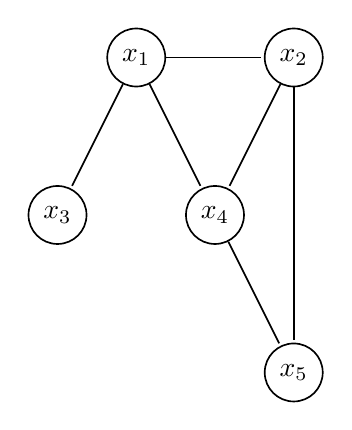
\begin{tikzpicture}[
    > = stealth, % arrow head style
    shorten > = 1pt, % space from node to arrow
    auto,
    node distance = 2cm, % distance between nodes
    semithick % line style
]

% Nodes
\node[draw, circle] (x1) at (0, 2) {$x_1$};
\node[draw, circle] (x2) at (2, 2) {$x_2$};
\node[draw, circle] (x3) at (-1, 0) {$x_3$};
\node[draw, circle] (x4) at (1, 0) {$x_4$};
\node[draw, circle] (x5) at (2, -2) {$x_5$};

% Edges
\draw[-] (x1) -- (x2);
\draw[-] (x1) -- (x3);
\draw[-] (x1) -- (x4);
\draw[-] (x2) -- (x4);
\draw[-] (x2) -- (x5);
\draw[-] (x4) -- (x5);

\end{tikzpicture}

We now prove Proposition 4.8 from more basic principles for completeness. We need to show that our assumed Markov blanket of X, consisting of X's parents, children and parents of X's children, is indeed d-separating X from all other nodes and is the minimal subset with this property. Firstly, note that all children and parents of X are trivially in the Markov blanket of X, since the direct edge they share with X ensures that they are dependent on X given any subset of the other nodes. Also, since when $Ch(X)$ is observed and therefore can form the center of a v-structure, all parents of these children are dependent on X given any superset of $Ch(X)$ (unless the parent itself is in the superset, which we observe is in conformity with our claim (Proposition 4.8) anyway). Thus, the Markov blanket of X at least contains all of these points. To showcase that this subset of nodes d-separates X from the rest of the graph, observe that any path cannot exit X upwards (as its parents are observed). Any path exiting X towards its children must go towards a parent of its children since $Ch(X)$ is observed and hence these nodes can only be centers of v-structures. But these parents are observed and hence these paths are blocked. 

\subsection{Part b}
$x_1 \independent x_2$ and $x_1 \independent x_2 | x_3$ are two CIs that hold in G but not in H.